\documentclass{beamer}

%\usetheme[framenumber,totalframenumber]{UniversiteitGent}
%\usetheme[faculty=di,framenumber,totalframenumber]{UniversiteitGent}
%\usetheme[faculty=we,usecolors,framenumber,totalframenumber]{UniversiteitGent}
%\usetheme[language=english,framenumber,totalframenumber]{AlleghenyCollege}
\usetheme{AnnArbor}
\usecolortheme{dove}

\title{CMPSC 390 \\ Blockchain Scalability.}
\author{Janyl Jumadinova}
\date{February 4, 2021}

\long\def\omitit#1{}

\usepackage{hyperref}
\hypersetup{
    colorlinks=true,
    linkcolor=blue,
    filecolor=magenta,      
    urlcolor=cyan,
}

\usepackage{color, soul}

\begin{document}

\begin{frame}
  \titlepage
\end{frame}

%%%%%%%%%%%% Slide %%%%%%%%%%%%%%%%%%%%%%%%%%%%%%%%%%%%%%%%%%%%%%%%%%%
\begin{frame}
  \frametitle{Scalability Problem}
	\begin{block}{\textbf{Goal}:}
		Provide all of the services that a blockchain offers to all users, independent of how many users there are.
	\end{block}
\end{frame}
%%%%%%%%%%%% Slide %%%%%%%%%%%%%%%%%%%%%%%%%%%%%%%%%%%%%%%%%%%%%%%%%%%
\begin{frame}
  \frametitle{Layer 1 vs. Layer 2}
	\begin{block}{\emph{Layer 1}:}
	\begin{itemize}
		\item refers to the main blockchain architecture
		\item the Bitcoin Blockchain, the Ethereum Blockchain
	\end{itemize}
	\end{block}
	\pause
	\begin{block}{\emph{Layer 2}:}
	\begin{itemize}
		\item refers to a secondary framework or protocol that is built on top of an existing blockchain
		\item the Lightning Network, Ethereum Plasma
	\end{itemize}
	\end{block}	
\end{frame}
%%%%%%%%%%%% Slide %%%%%%%%%%%%%%%%%%%%%%%%%%%%%%%%%%%%%%%%%%%%%%%%%%%
\begin{frame}
  \frametitle{Taproot (Layer 1)}
 {\tiny{ \url{https://www.coindesk.com/taproot-merged-bitcoin-core}}} \\
 \pause
  \textbf{Problems}:
 \begin{itemize}
 	\item Signature verification is slow, but required everywhere in the network.
%case 1: when validating a new block
%case 2: when a node newly connects (or reconnects) to the network
	\item Users can see many details of a transaction (all scripts, multisignature, etc.)
  \end{itemize}
  \pause
  \textbf{Taproot + Schnorr}
	\begin{itemize}
		\item \textcolor{brown}{Schnorr} is a type of signature, \textcolor{brown}{Taproot} is the Bitcoin upgrade (BIP) that uses Schnorr. \pause
		\item \textbf{Idea}: If signature validation is faster, much of the network can run faster (more throughput). \pause
		\item Taproot replaces ECDSA signatures with Schnorr Signatures.
	\end{itemize}
\end{frame}
%%%%%%%%%%%% Slide %%%%%%%%%%%%%%%%%%%%%%%%%%%%%%%%%%%%%%%%%%%%%%%%%%%
\begin{frame}
  \frametitle{Benefits of Taproot + Schnorr}
	\begin{block}{\emph{Key aggregation}:}
	\begin{itemize}
		\item Multiple signers create an aggregate public key and an aggregate signature. \pause
		\item Multisig looks and costs the same as a single signature. \pause
		\item $30-75\%$ savings. 
	\end{itemize}
	\end{block}
	\pause
	\begin{block}{\emph{Batch validation}:}
	\begin{itemize}
		\item Many signatures can be verified at once. \pause
		\item Speedup grows logarithmically with the number of sigs to verify. \pause
		\item When a transaction has many scripts, they do not need to be revealed or evaluated on the network. 
	\end{itemize}
	\end{block}
\end{frame}
%%%%%%%%%%%% Slide %%%%%%%%%%%%%%%%%%%%%%%%%%%%%%%%%%%%%%%%%%%%%%%%%%%
\begin{frame}
  \frametitle{Segregated Witness (Layer 1)}
{\tiny{\url{https://blockchainhub.net} by Valentik Kalinov}}
 	\centering
	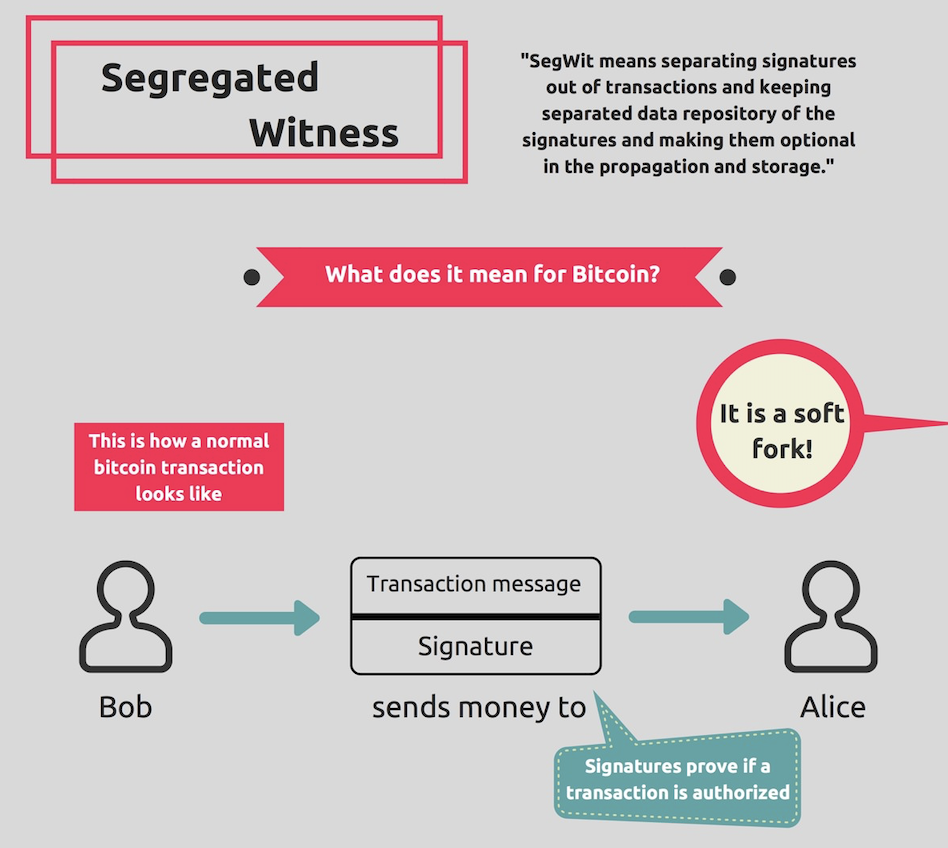
\includegraphics[scale=0.45]{segwit1}
\end{frame}

%%%%%%%%%%%% Slide %%%%%%%%%%%%%%%%%%%%%%%%%%%%%%%%%%%%%%%%%%%%%%%%%%%
\begin{frame}
  \frametitle{Segregated Witness}
 	\centering
	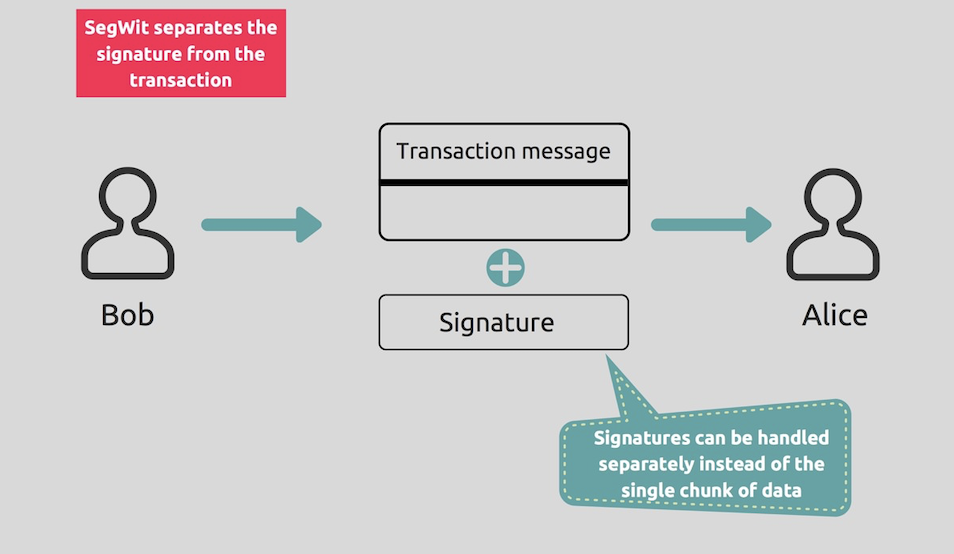
\includegraphics[scale=0.6]{segwit2}
\end{frame}
%%%%%%%%%%%% Slide %%%%%%%%%%%%%%%%%%%%%%%%%%%%%%%%%%%%%%%%%%%%%%%%%%%
\begin{frame}
  \frametitle{Segregated Witness}
 	\centering
	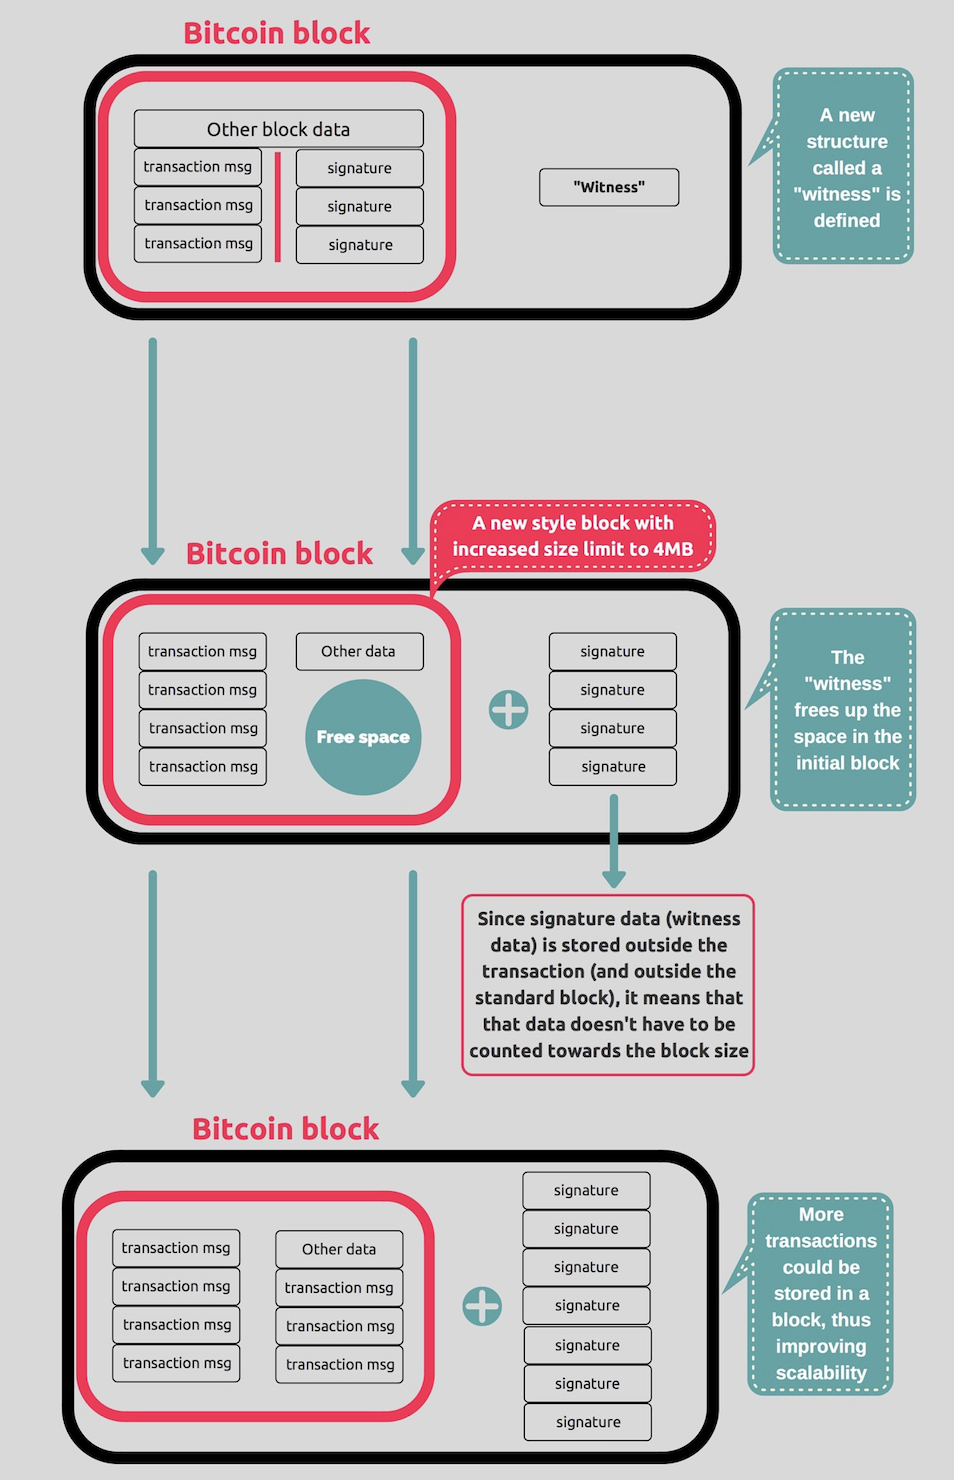
\includegraphics[scale=0.3]{segwit3}
\end{frame}
%%%%%%%%%%%% Slide %%%%%%%%%%%%%%%%%%%%%%%%%%%%%%%%%%%%%%%%%%%%%%%%%%%
\begin{frame}
  \frametitle{Sharding}
  \begin{block}{\textcolor{brown}{Sharding:}} 
  Do not require every miner to be working on every single block, essentially creating parallel but connected blockchains.
  \end{block}
  \pause	
  
 	\centering
	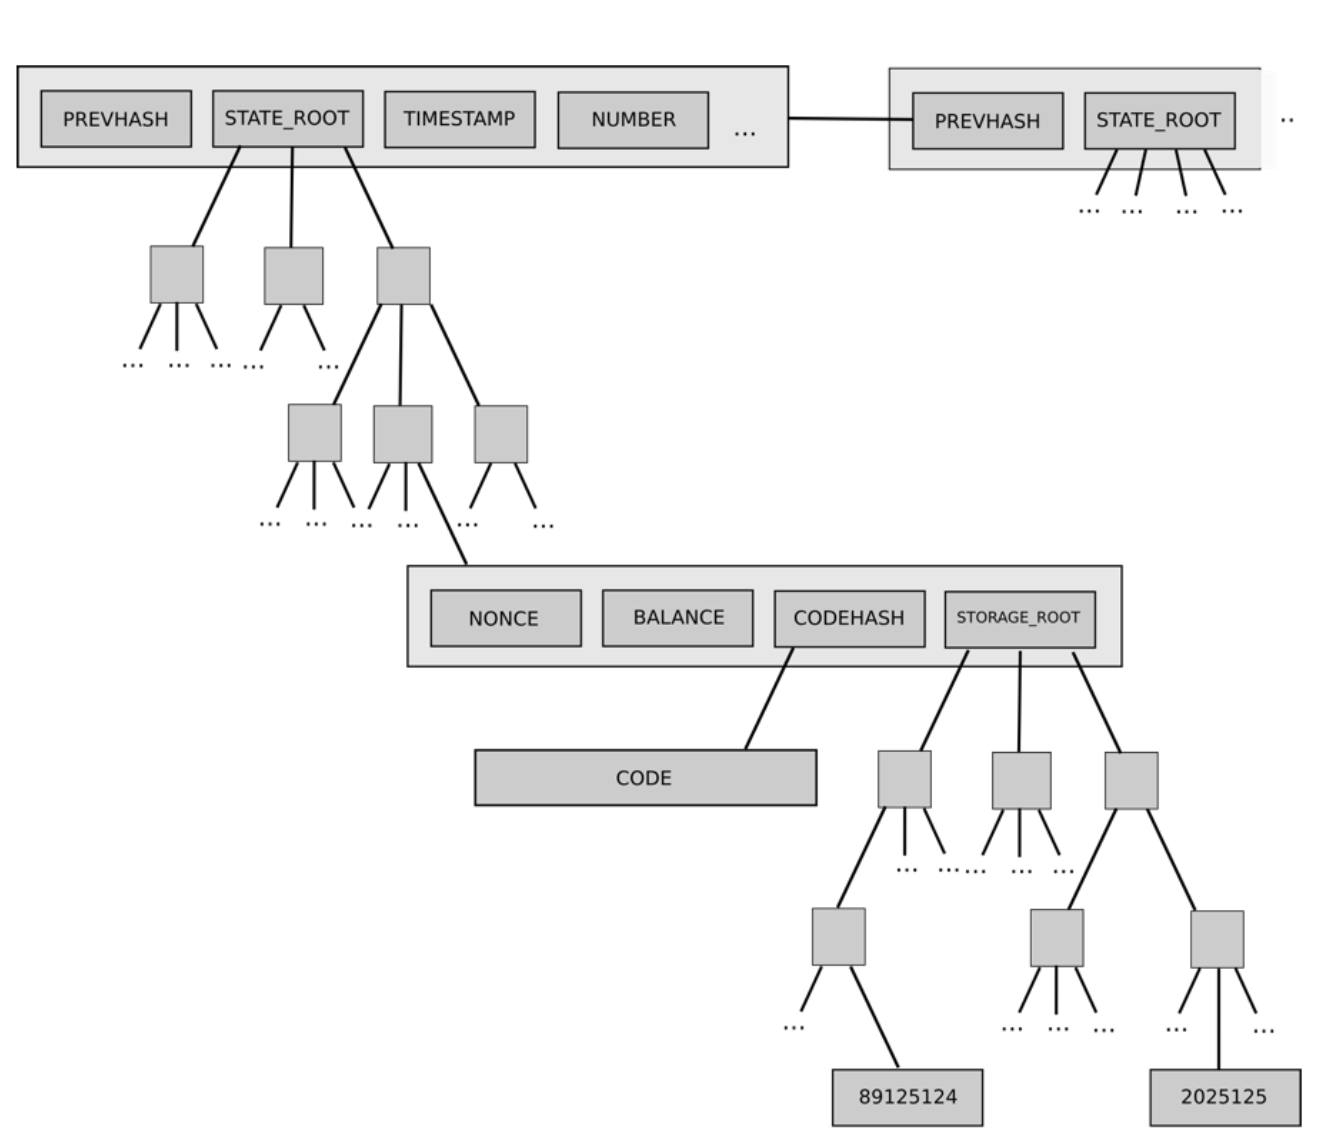
\includegraphics[scale=0.23]{sharding} \\
{\tiny{Ref.: \url{https://eth.wiki/sharding/Sharding-FAQs}}}
\end{frame}
%%%%%%%%%%%% Slide %%%%%%%%%%%%%%%%%%%%%%%%%%%%%%%%%%%%%%%%%%%%%%%%%%%
\begin{frame}
  \frametitle{Lightning Network (Layer 2)}
  \url{https://lightning.network/}
  \pause
  \begin{block}{\textcolor{brown}{Lightning Network}}
  Do not put every transaction on the blockchain.
  \end{block}
 \pause
 \textbf{Payment Channel}	
 \centering
	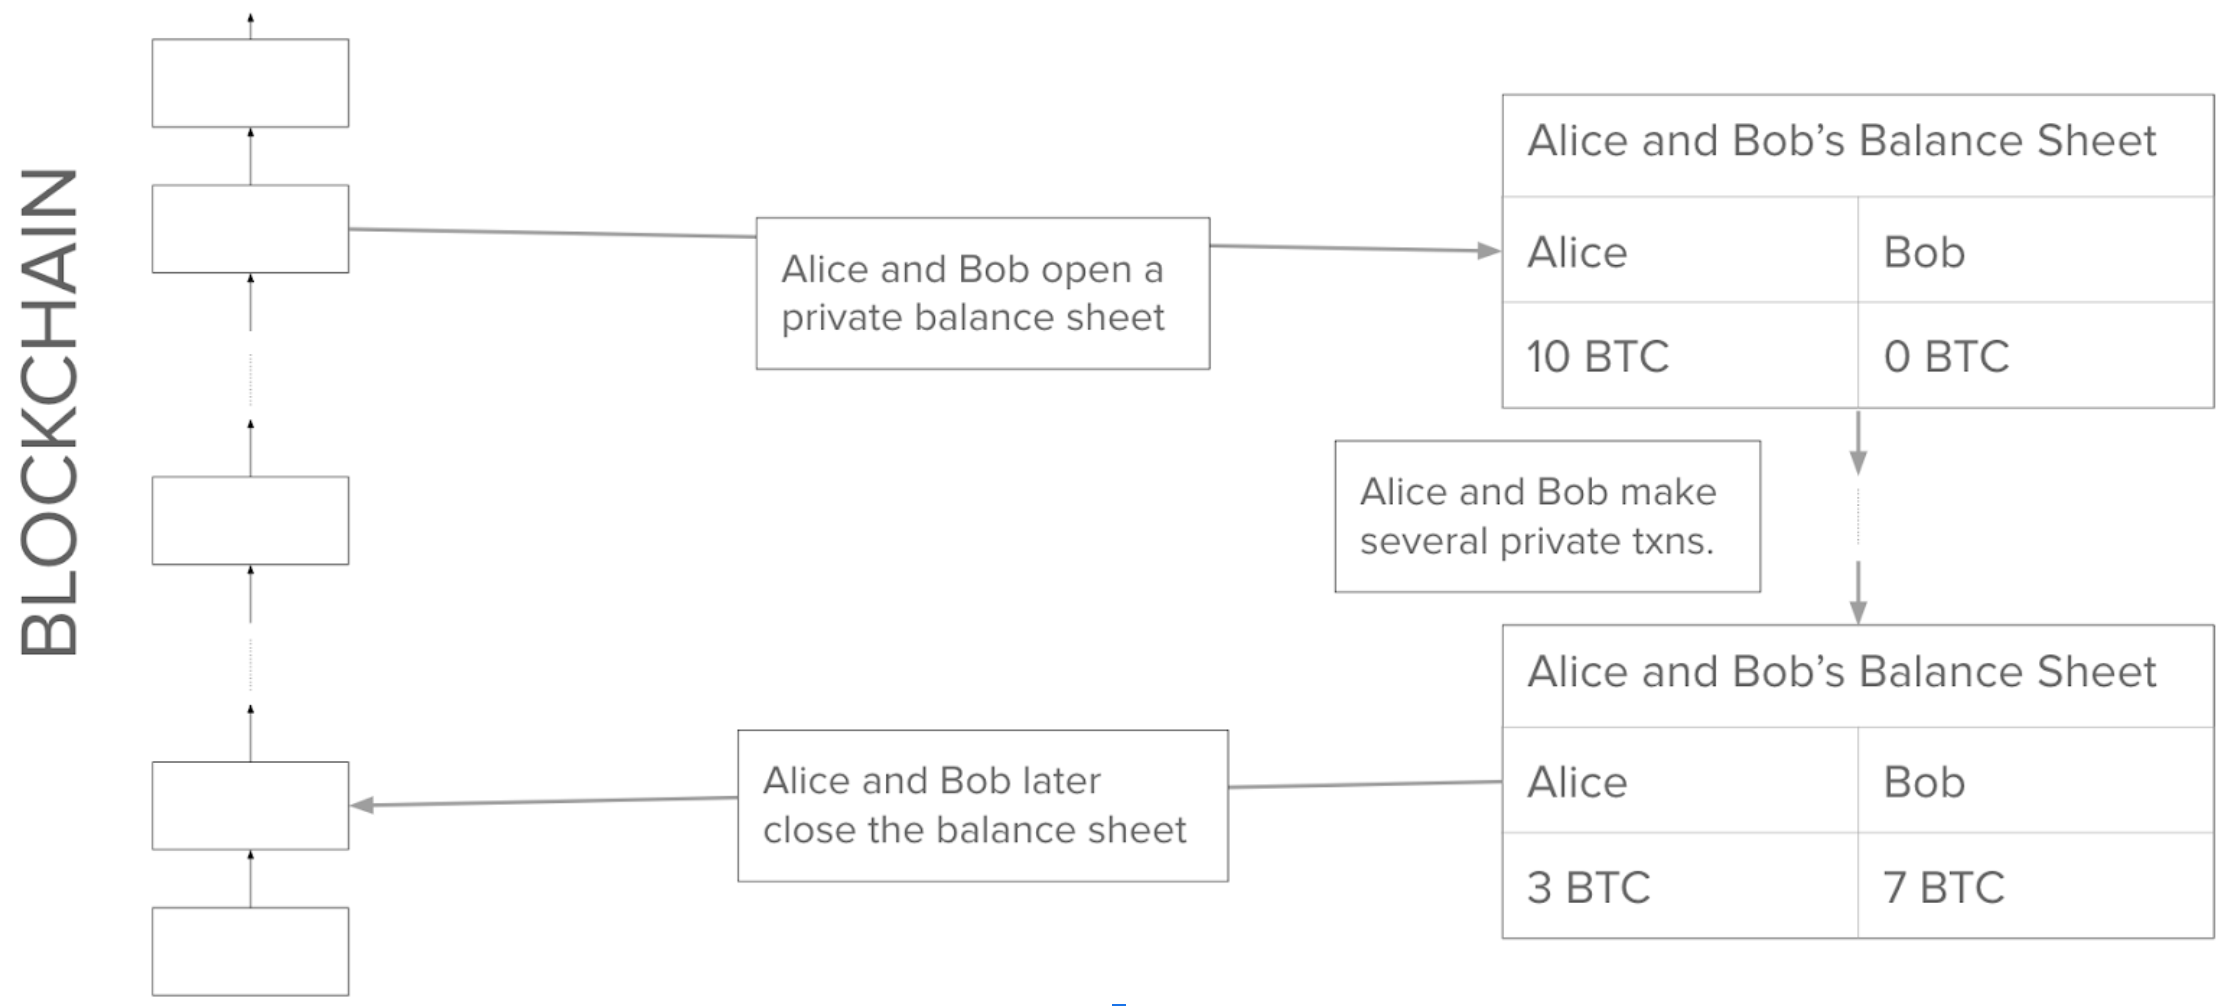
\includegraphics[scale=0.23]{payment}
\end{frame}
%%%%%%%%%%%% Slide %%%%%%%%%%%%%%%%%%%%%%%%%%%%%%%%%%%%%%%%%%%%%%%%%%%
\begin{frame}
  \frametitle{Lightning Network}
  \url{https://lightning.network/}
 \centering
	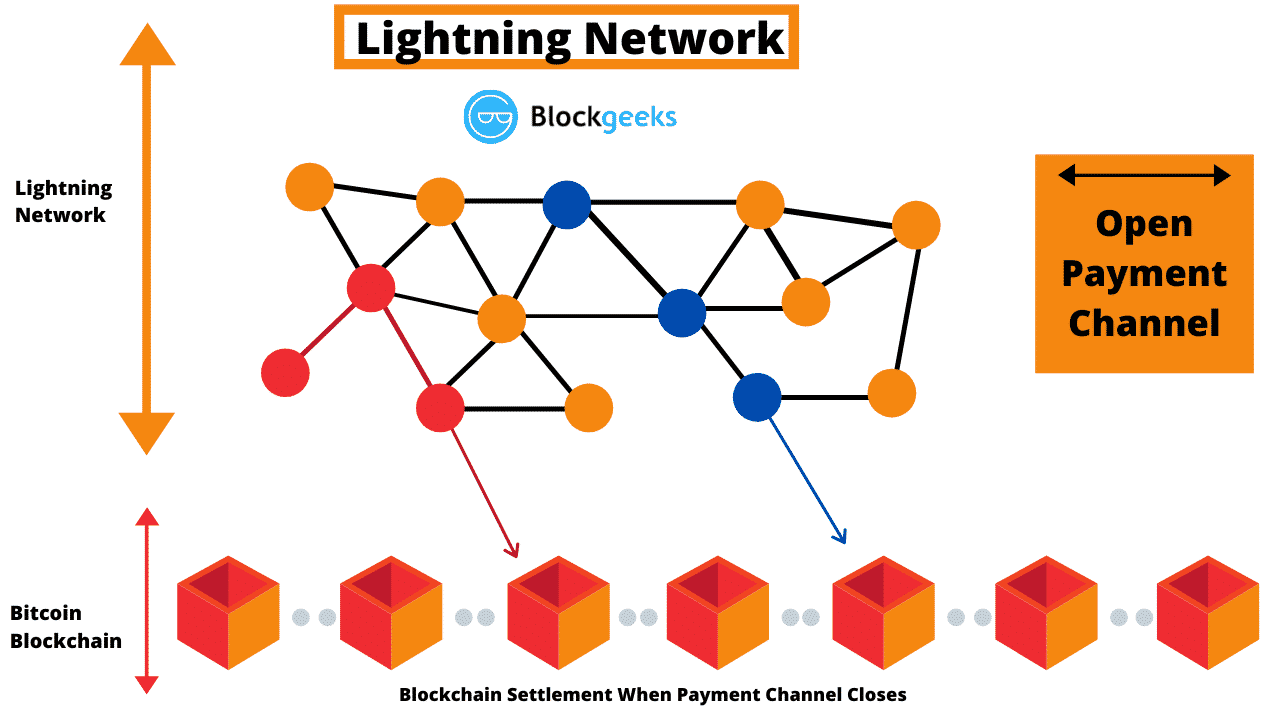
\includegraphics[scale=0.3]{LN}
\end{frame}
%%%%%%%%%%%% Slide %%%%%%%%%%%%%%%%%%%%%%%%%%%%%%%%%%%%%%%%%%%%%%%%%%%
\begin{frame}
  \frametitle{Ethereum 2.0}
 \centering
	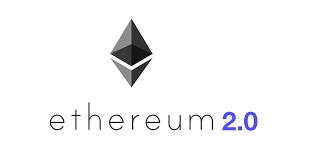
\includegraphics[scale=0.35]{eth} \\
	
  Multi-year timeline. 
 	\begin{itemize}
 		\item \emph{Phase 0}: Transition to Proof of Stake.
 		\item \emph{Phase 1}: Data Sharding.
 		\item \emph{Phase 2}: State + Execution (computation and smart contracts).
 		\item \emph{Phase 3+}: Other scaling solutions.
 	\end{itemize}
\end{frame}
%%%%%%%%%%%% Slide %%%%%%%%%%%%%%%%%%%%%%%%%%%%%%%%%%%%%%%%%%%%%%%%%%%
\end{document}
